\section{Données}
\label{sec:data}

\subsection{Jeu de données}

Le jeu de données utilisé est CUB-200-2011~\cite{wah2011cub}
(Caltech-UCSD Birds), qui comprend 11\,788 images réparties sur 200
espèces d'oiseaux. La distribution du nombre d'images par classe est
légèrement déséquilibrée, avec un minimum de 41 images et un maximum de 60
images par classe (Figure~\ref{fig:class_distribution}), ce qui ne
nécessite pas de pondération de classes particulière. Les images ont une
résolution native moyenne de 471$\times$384 pixels, avec une variabilité
notable (de 140 à 500 pixels de large selon les images), ce qui justifie
le choix d'un redimensionnement systématique à 224$\times$224 pixels pour
l'entraînement.

\begin{figure}[t]
  \centering
  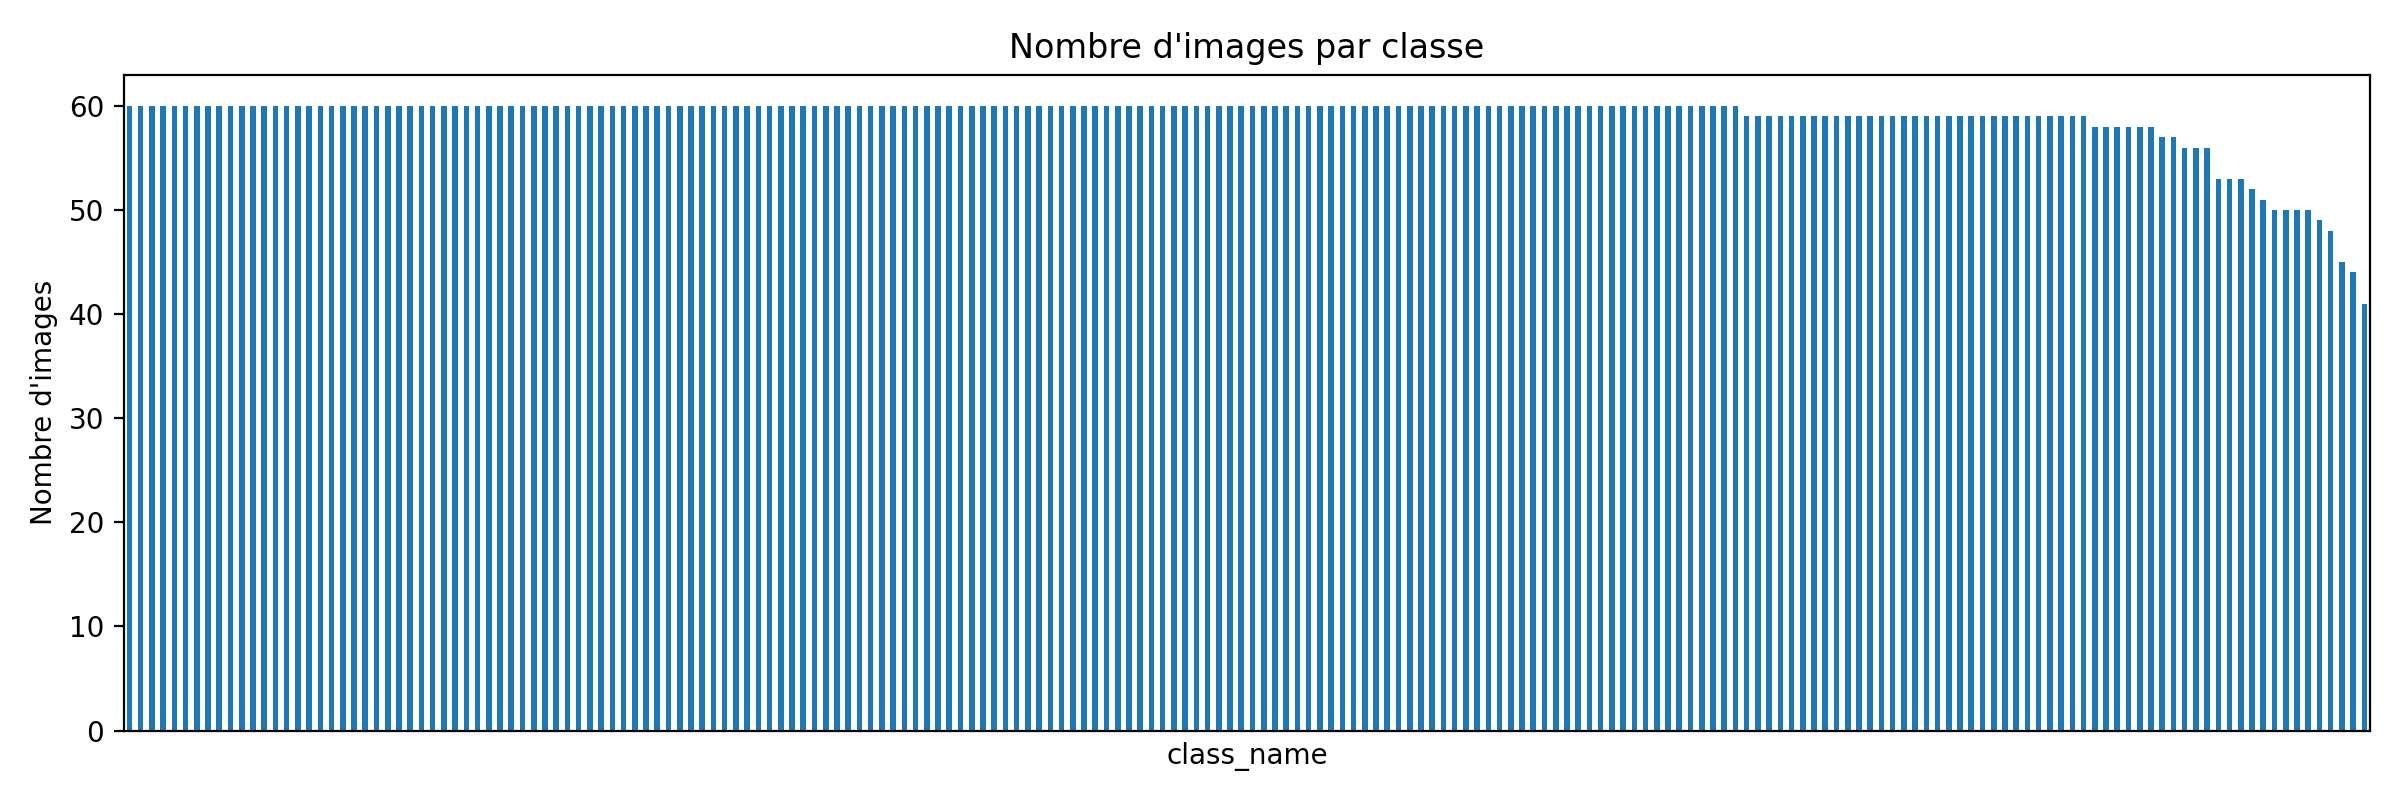
\includegraphics[width=\linewidth]{../data/data_processed/figures/eda_class_distribution.png}
  \caption{Distribution du nombre d'images par classe sur CUB-200-2011.}
  \label{fig:class_distribution}
\end{figure}

La Figure~\ref{fig:similar_classes} illustre la difficulté propre à la
classification fine-grained : plusieurs espèces de moineaux (\emph{Baird
Sparrow}, \emph{Black-throated Sparrow}, \emph{Brewer Sparrow},
\emph{Chipping Sparrow}) partagent une silhouette et une taille très
proches, et ne se distinguent que par des détails de plumage.

\begin{figure}[t]
  \centering
  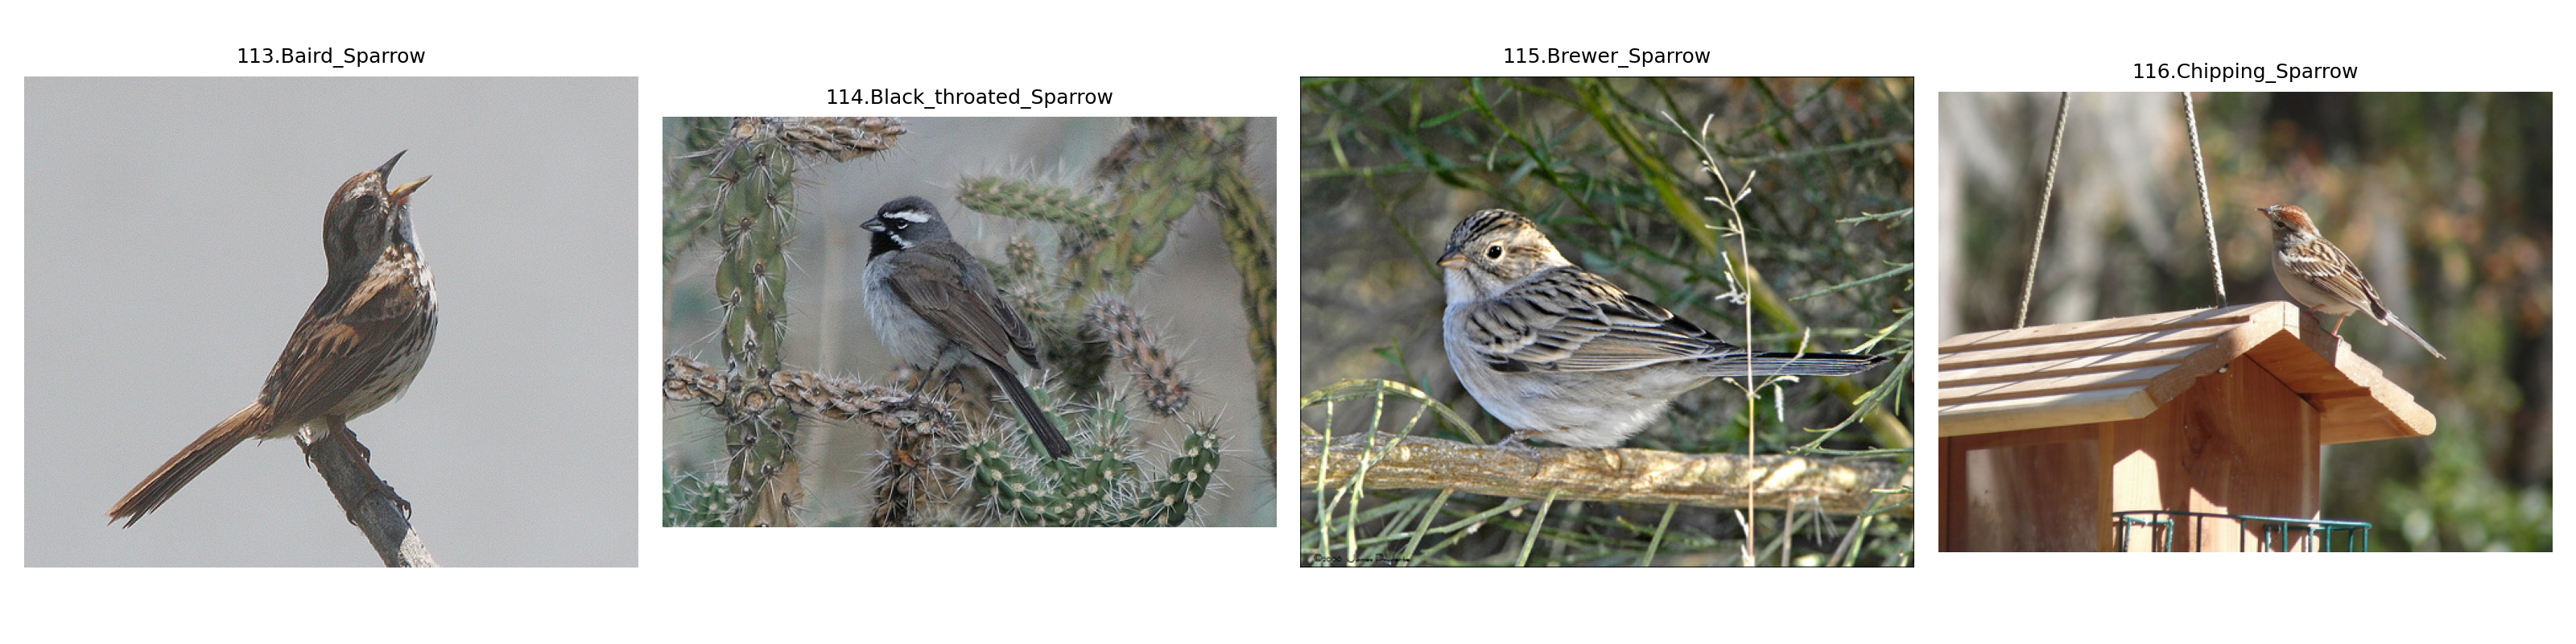
\includegraphics[width=\linewidth]{../data/data_processed/figures/eda_similar_classes.png}
  \caption{Exemple de classes visuellement proches (famille des moineaux), illustrant la difficulté du fine-grained.}
  \label{fig:similar_classes}
\end{figure}

\subsection{Prétraitement}

Toutes les images sont redimensionnées à 224$\times$224 pixels et
normalisées avec les statistiques d'ImageNet (moyenne et écart-type par
canal RGB), afin d'assurer la compatibilité avec les modèles
pré-entraînés utilisés (Section~\ref{sec:methodology}).

\subsection{Séparation train / validation / test}

Le split officiel de CUB-200-2011 fournit une séparation
train/test de 5\,994 / 5\,794 images. À partir de l'ensemble
d'entraînement officiel, un sous-ensemble de validation stratifié de
15\,\% est extrait (seed fixe = 42), aboutissant à la répartition finale
suivante :

\begin{table}[t]
  \centering
  \caption{Répartition finale des images par split.}
  \label{tab:splits}
  \begin{tabular}{lc}
    \toprule
    Split & Nombre d'images \\
    \midrule
    Train & 5\,094 \\
    Validation & 900 \\
    Test & 5\,794 \\
    \midrule
    Total & 11\,788 \\
    \bottomrule
  \end{tabular}
\end{table}

\subsection{Sous-échantillonnage pour l'analyse data-hungry}

Afin d'étudier la sensibilité de chaque architecture à la quantité de
données d'entraînement (Section~\ref{sec:ablation}), quatre
sous-ensembles stratifiés de l'ensemble d'entraînement sont générés,
correspondant à 10\,\%, 25\,\%, 50\,\% et 100\,\% des 5\,094 images de
train (seed fixe = 42, toutes les 200 classes restant représentées même
dans le sous-ensemble à 10\,\%).

\subsection{Augmentation des données}

Deux pipelines d'augmentation sont définis pour l'entraînement : un
pipeline \emph{faible} (retournement horizontal aléatoire, recadrage
aléatoire léger) et un pipeline \emph{fort} (ajout d'une variation
colorimétrique, d'une rotation aléatoire et d'un effacement aléatoire de
zones de l'image). Aucune augmentation n'est appliquée sur les ensembles
de validation et de test.